\documentclass[journal]{IEEEtran}

\usepackage{cite,graphicx}
\usepackage[usenames,dvipsnames]{xcolor}

% *** GRAPHICS RELATED PACKAGES ***
%
\ifCLASSINFOpdf
  % \usepackage[pdftex]{graphicx}
  % declare the path(s) where your graphic files are
  % \graphicspath{{../pdf/}{../jpeg/}}
  % and their extensions so you won't have to specify these with
  % every instance of \includegraphics
  % \DeclareGraphicsExtensions{.pdf,.jpeg,.png}
\else
  % or other class option (dvipsone, dvipdf, if not using dvips). graphicx
  % will default to the driver specified in the system graphics.cfg if no
  % driver is specified.
  % \usepackage[dvips]{graphicx}
  % declare the path(s) where your graphic files are
  % \graphicspath{{../eps/}}
  % and their extensions so you won't have to specify these with
  % every instance of \includegraphics
  % \DeclareGraphicsExtensions{.eps}
\fi

\usepackage{graphicx}
\usepackage[cmex10]{amsmath}
\usepackage{algorithmic}
\usepackage{array}
\usepackage{mdwmath}
\usepackage{mdwtab}
\usepackage{eqparbox}
%\usepackage[tight,footnotesize]{subfigure}
%\usepackage[caption=false]{caption}
%\usepackage[font=footnotesize]{subfig}
%\usepackage[caption=false,font=footnotesize]{subfig}
\usepackage{fixltx2e}
\usepackage{stfloats}
\usepackage{url}

% *** Do not adjust lengths that control margins, column widths, etc. ***
% *** Do not use packages that alter fonts (such as pslatex).         ***
% There should be no need to do such things with IEEEtran.cls V1.6 and later.
% (Unless specifically asked to do so by the journal or conference you plan
% to submit to, of course. )

% correct bad hyphenation here
\hyphenation{op-tical net-works semi-conduc-tor}

\begin{document}
%
% paper title
% can use linebreaks \\ within to get better formatting as desired
\title{TODO: A Survey of StarCraft AI Techniques}
%
%
% author names and IEEE memberships
% note positions of commas and nonbreaking spaces ( ~ ) LaTeX will not break
% a structure at a ~ so this keeps an author's name from being broken across
% two lines.
% use \thanks{} to gain access to the first footnote area
% a separate \thanks must be used for each paragraph as LaTeX2e's \thanks
% was not built to handle multiple paragraphs
%

\author{FirstName~LastName,~\IEEEmembership{Member,~IEEE,}
        Jim~Raynor,~\IEEEmembership{Fellow,~RR,}
        and~Sarah~Kerrigan,~\IEEEmembership{Life~Fellow,~ZS}% <-this % stops a space
\thanks{FirstName~LastName is with the Department of Names
GA, 30332 USA e-mail: (see http://www.michaelshell.org/contact.html).}% <-this % stops a space
\thanks{J. Raynor and S. Kerrigane are with the Romeo\&Juliet Inc.}% <-this % stops a space
\thanks{Manuscript received April 19, 2499; revised January 11, 2500.}}

% note the % following the last \IEEEmembership and also \thanks - 
% these prevent an unwanted space from occurring between the last author name
% and the end of the author line. i.e., if you had this:
% 
% \author{....lastname \thanks{...} \thanks{...} }
%                     ^------------^------------^----Do not want these spaces!
%
% a space would be appended to the last name and could cause every name on that
% line to be shifted left slightly. This is one of those "LaTeX things". For
% instance, "\textbf{A} \textbf{B}" will typeset as "A B" not "AB". To get
% "AB" then you have to do: "\textbf{A}\textbf{B}"
% \thanks is no different in this regard, so shield the last } of each \thanks
% that ends a line with a % and do not let a space in before the next \thanks.
% Spaces after \IEEEmembership other than the last one are OK (and needed) as
% you are supposed to have spaces between the names. For what it is worth,
% this is a minor point as most people would not even notice if the said evil
% space somehow managed to creep in.

% The paper headers
\markboth{TCIAIG ~Vol.~X, No.~Y, Month~Year}%
{Shell \MakeLowercase{\textit{et al.}}: TODO: Title here}

\maketitle

\begin{abstract}
TODO: Idea of the paper is: ``one-stop guide on what is the
state of the art in Starcraft AI''. It should help people participating in the competition focus
their efforts, and also should help people implementing AI for RTS games in
general (e.g. industry).  In Gabriel's words ``RTS AI problems, Solutions, State-of-the-art, conclude on what's "solved" since \cite{Buro03rts} and what's not.'' 

For example, if someone wants to implement a bot, and wonders "how should I do scouting", our paper should provide a summary of the existing techniques, and pointers to know more. 
\end{abstract}

\begin{IEEEkeywords}
Game AI, Real-Time Strategy, Starcraft, Review1

\end{IEEEkeywords}

% For peer review papers, you can put extra information on the cover
% page as needed:
% \ifCLASSOPTIONpeerreview
% \begin{center} \bfseries EDICS Category: 3-BBND \end{center}
% \fi
%
% For peerreview papers, this IEEEtran command inserts a page break and
% creates the second title. It will be ignored for other modes.
\IEEEpeerreviewmaketitle

\section{Introduction}\label{sec:intro}
\IEEEPARstart{S}{ince} Michael Buro's call for research in RTS games \cite{Buro03rts}, many researchers have answered the call. Specially, AI competitions like the Starcraft one have caused many AI techniques to be
applied to RTS AI. We will list and classify these approaches, explain their 
power and their downsides and conclude on what is left to achieve human-level 
RTS AI.

{\color{blue}
Motivate the paper, and provide an outline.

Some arguments to use in the motivation could be that games are a good application to motivate novel AI research (as has been happening throughout the history of AI), and that techniques and algorithms developed for RTS games, in addition to be useful and relevant to the game industry, have broader application to other areas.

Reiterate that the goal of this paper is to provide a one-stop guide on what is the
state of the art in Starcraft AI
}

\section{Real-Time Strategy Games}\label{sec:rts}

\subsection{Starcraft}\label{subsec:starcraft}

Starcraft: Brood War is a popular RTS game released in 1998 by Blizzard Entertainment. Starcraft is set in a science-fiction based world where the player must choose one of the three races: Terran, Protoss or Zerg. The good work done by the people of Blizzard makes this game one of the most extremely well-balanced RTS games ever created.
\begin{itemize}
	\item Terrans, human exiled from Earth, provide units that are versatile and flexible giving a balanced option between Protoss and Zergs.
	\item Protoss units have lengthy and expensive manufacturing process, but they are strong and resistant. These conditions makes players follow a strategy of quality over quantity.
	\item Zergs, the insectoid race, units are cheap and weak. They can be produced fast, encouraging players to overwhelm their opponents with sheer numbers.
\end{itemize}

\subsection{Challenges in RTS Game AI}\label{subsec:challenges}

{\color{blue}
This section should be brief, and just give us some basic ideas of which are the challenges in RTS Game AI, so that when we refer to related work, we can use this as a reference point.  The most important thing of this section is to demonstrate that RTS games are complex.

Many years have passed since Buro's call for research (8!!). he identified 6 challenges:
\begin{itemize}
\item Resource management
\item Decision making under uncertainty
\item Spatial and temporal reasoning
\item Collaboration
\item Opponent modeling, Learning
\item Adversarial real-time planning
\end{itemize}

There has been a lot of work in many, but others have been untouched (e.g. Collaboration). Additionally, other challenges that are not in the list appeared, and have been worked on, like: how to exploit the existing domain knowledge (strategies, build-orders, replays, etc.), or how to design an architecture that integrates all the modules required for an agent to play an RTS games. 

\begin{itemize}
\item Task Decomposition (or ``Architecture'')
\item Integration of Domain Knowledge
\item Reasoning with Uncertainty (including information gathering)
\item Opponent Modeling and Adaptation: opponent modeling is key if we have to adapt our strategy. As different strategies are dominating each others, forming multiple Nash equilibria, the AI has to be able to infer the intend of its opponent.
\item Group and Individual Control (``micro''): the task of controlling units efficiently (we can not speak of optimality here due to the huge state space, and of the enemy behavior entails numerous Nash equilibria), focusing fire to diminish enemy's firepower and keeping our units alive the longest, casting defensive and offensive spells and abilities.
\item Planning and Resource Allocation (``macro'')
\item Spatial reasoning (``tactics'')
\end{itemize}

Maybe the list above goes better in Section \ref{sec:questions}?
}


\section{Existing work on RTS Game AI}\label{sec:review}


\subsection{Perception}
Every AI needs to observe the world in order to analyze it and take decisions. In RTS games this task isn't trivial since we have to deal with imperfect information.

\textbf{Spatial}

Terrain analysis supplies the AI with chunks of abstract information about the map in order to help in making decisions. This analysis is usually performed off-line, in order to save processing time during gameplay.

Pottinger \cite{Pottinger00} described \emph{BANG!} engine implemented by Ensemble Studios for the game Age of Empires 2. This engine provides terrain analysis functionalities to the game using influence maps and areas with connectivity information. Later works \cite{Forbus01} showed the importance to have qualitative spatial information, and some others \cite{Karavelas04}\cite{Hale08} focused on spatial decomposition. The most recent work \cite{Perkins10} presented an algorithm using Voronoi diagrams to detect regions and relevant choke points.

\textbf{Temporal}

In \cite{WeberAIIDE11} a particle model is used to tracks opponent units under fog of war over time.

{\color{ForestGreen}
Anyone did anything here? I think only Skynet uses temporal reasoning...
Maybe heat maps?? but I can't find any reference...
}

\textbf{Enemy}

Opponent modeling is the process of keeping track of what the enemy is doing during a game in order to estimate the probability of it using a specific strategy.

The main methods used to these ends are case-based reasoning (CBR) and planning or plan recognition \cite{LTW,CBR_Planning,OntanonCBR,HTNPlanning,Ramirez}.\cite{LTW} used CBR to perform dynamic plan retrieval extracted from domain knowledge in Wargus (Warcraft II clone). \cite{CBR_Planning} base their real-time case-based planning (CBP) system on a plan dependency graph which is learned from human demonstration. In \cite{OntanonCBR,PlanRetrieval}, they use CBR and expert demonstrations on Wargus. They update their previous CPB approach by using ``situation assessment'' for plan retrieval. They improve the speed of CPB by using a decision tree to select relevant features. Hsieh and Sun \cite{HsiehS08} based their work on \cite{LTW} CBR model and used StarCraft replays to construct states and building sequences. Strategies are choices of building construction order in their model. 

\cite{SchaddBS07} describe opponent modeling through hierarchically structured models of the opponent behavior and they applied their work to the Spring RTS (Total Annihilation clone). \cite{HTNPlanning} use hierarchical task networks (HTN) to model strategies in a first person shooter with the goal to use HTN planners. \cite{OBRecog} improve the probabilistic hostile agent task tracker (PHATT \cite{PHATT}, a simulated HMM for plan recognition) by encoding strategies as HTN. %\cite{Madeira06} 
\cite{WeberCig09} proposed ``a data mining approach to strategy prediction'' and performed supervised learning on StarCraft replays. \cite{HMMstrat_RTS_AIIDE11} used HMM to learn the transition probabilities of sequences of constructions and kept the most probables to produce probabilistic behavior models (in StarCraft). \cite{SynnaeveOpeningCig11} continued on \cite{WeberCig09} and used a Bayesian semi-supervised (labeling based on clustering) model to learn from replays and predict openings (early game strategies) from StarCraft replays, while \cite{SynnaeveAIIDE11} presents a whole game Bayesian tech-tree predictor based on unsupervised learning from replays.

Most commercial games avoid gather this information making their AI omniscient and using perfect information all the time. But sometimes they simulate some scouting tasks as Bob Fitch described in his AIIDE 2011 keynote for the game series WarCraft and StarCraft I.

{\color{ForestGreen}
Nobody had described an efficient way to scout the opponent... better opponent information better opponent modeling...
}

\textbf{Ally}

{\color{ForestGreen}
Anyone did anything here?
}

\subsection{Strategy}

The most common decision making are Decision Trees. Some of the advantages of the decision trees are: simple to understand and interpret acting like a white box where we can explain why a decision is taken, and they are compatible with other decision techniques. For complex decisions we have many algorithms to generate an optimum decision tree like ID3 or C4.5, depends on the problem we will use one or another.

A good alternative are Finite State Machine. The idea behind FSM is to decompose an object's behavior into easily manageable "chunks" or states, such as "attacking an enemy", "gathering resources" or "repairing" and establish the conditions that trigger transitions between them.

\subsection{Giving orders}

{\color{ForestGreen}
Explain centralized models (like blackboard) and distributed/hierarchically models.
}

\subsection{Executing orders}

\textbf{Pathfinding}

The most common pathfinding algorithm is A*, but the big problem of this algorithm is the time and  memory consumption, a show-stopper in a real-time environment.

To solve this the search space needs to be reduced as much as possible. One common technique is reducing the tile map search into a navigation graph map. To do this some polygonal triangulations are calculated and abstracted on a grid-based map and this is the TRA* (Triangulation Reduction A*) algorithm\cite{Demyen_2006}. 

{\color{ForestGreen}
There are a lot of new pathfinding algorithms. Do we need to review all of them?
}

\textbf{Group behavior}

Craig Reynols introduced algorithmic steering behaviors to simulate the aggregate motion of swarms using procedural animation\cite{Reynolds_1999}. His model describes how a system of multiple agents , each steering according to simple local rules, can produce the collective movement found in flocks of birds. With this behaviours we are able to simulate intelligent squad movements and do tactical moves to flank the opponent in a RTS game\cite{Danielsiek_2008}, improving the survival of our units.

A good alternative to Flocking is using Reciprocal Velocity Obstacles (RVO)\cite{Berg_2008}, since it is easier to control the behavior and they guarantee to prevent collisions. With this algorithm we can move a large squad crossing another squad and avoid all possible collisions between units. This type of techniques are already applied in commercial RTS games like Starcraft 2 or Supreme Commander 2 with great success.

Another popular technique is Potential Fields. basically, Potential Fields work like a charged particle moving through a magnetic field. The process of tuning and optimizing the parameters of potential field charges can be time reduced applying learning algorithms such as Q-Learning\cite{Liu_2008}. Another common issue we have to deal with when using potential fields is the local optima problem that can stuck the unit away from the goal. Some examples of the utilities of potential files in RTS games are avoiding obstacles (navigation), avoiding opponent fire, or staying at maximum shooting distance\cite{Hagelback08,Hagelback09}.

There are some interesting uses of reinforcement learning (RL) \cite{Sutton}: \cite{Marthi05} employs concurrent hierarchical Q-learning (units Q-functions are combined at the group level) RL to efficiently control units in a ``one robot with multiple effectors'' fashion. \cite{Madeira06} advocates the use of prior domain knowledge to allow faster RL learning and applied their work on a turn-based strategy game. In real game setups, the actions spaces to explore is gigantic, it requires to use the structure of the game in a partial program (or a partial Markov decision process) and a shape function (or a heuristic) \cite{Marthi05}. There are other was to learn parameters of an underlying model, for instance \cite{GA} used evolutionary learning techniques, but face the same problem of dimensionality. The difficulty to work with multi-scale goals and plans is handled directly by case-based reasoning (CBR), which has been adapted for units behavior with continuous action models \cite{Molineaux08}, an integrated RL/CBR algorithm using continuous models, or with hybrid CBR/RL transfer learning \cite{CBR-RL}. Reactive planning (for behavior languages) \cite{WeberCig10}, a decompositional planning similar to hierarchical task networks \cite{HTNPlanning}, allows for plans to be changed at different granularity levels and so for multi-scale (hierarchical) goals integration.

Self-organizing-maps (SOM) learned with evolutionary algorithms provide some way to learn (realistic) parameters for RTS units behavior \cite{teamCompositionRTS}. Bayesian programming has been applied to inverse fusion of the sensory inputs of the units \cite{SynnaeveMicroCig11}, which subsumes potential fields, allowing for integration of tactical goals directly in micro-management. There are also some cognitive approaches to RTS AI \cite{SORTS}, in which there is a human-like attention model for micro-management.



%\subsection{Integration of Domain Knowledge}\label{subsec:domainknowledge}

{\color{blue}
All bots attempt at integrating human domain knowledge in a way or another, be it in the form of build-orders, heuristics, strategies, or by automatically learning from human replays. This has been shown to be key to good performance in bots (for now, as Dave was saying: ``Starcraft AI is like Chess was in the 60s''). 

Talk about learning, scripting, and other techniques to incorporate such knowledge.


When talking about learning in RTS games, with regard to a particular match against an opponent, one has to differentiate between:
\begin{itemize}
\item prior learning: done before the match, like when a bot learns what is likely to happen on a given match-up (and map) from replays, or when a bot optimizes its micro-management parameters through simulated annealing or genetic evolution.
\item in-match learning: done between the different games of match, ``the opponent rushed me last game so I will play this one safe''.
\item in-game learning: done between the different actions of the game, ``I tried to attack here and it was a failure, let us try somewhere else''.
\end{itemize}
All these learning can be supervised (labeled replays, scripted situations) or unsupervised (unlabeled data, exploratory situations). The last two kinds of situations of learning are more inclined towards reinforcement learning because the AI has to deal with the exploration-exploitation duality. %prior learning: supervised \cite{WeberCIG09} \cite{SynnaeveCIG11}, unsupervised: \cite{SynnaeveAIIDE11}
}

%\subsection{Reasoning with Uncertainty}\label{subsec:uncertainty}

{\color{blue}
I think there are two important aspects of uncertainty in RTS games:
\begin{itemize}
\item First is trying to model uncertainty and try to reduce it (information gathering, and representation of knowledge), this includes scouting, and maintaining good estimates of locations and number of units of the enemy, etc.
\item Second is actually using the uncertain information. Taking decisions like army strength estimation (like to attack or retreat).
\end{itemize}

There are two main kinds of uncertainty, existing for two different reasons, in RTS games. First, there is the incompleteness of information, due to the fog of war, which leads to some kind of ``extensional'' 
%``extensive'' 
uncertainty, that can be lowered by good scouting, and knowledge representation and reasoning (to infer what is possible given what has been seen). Also, there is the fact that we will never be able to read the opponent's mind, the ``intentional'' 
%or ``intensive'' 
uncertainty that we can't really be sure to scratch off, even with the best scouting possible. For intentional uncertainty, the AI, as the human player, can only build a sensible model of what the opponent is likely to do, to think, or to think knowing what we think he thinks. Both these kinds of uncertainty can be studied through probabilities, but only $P(Hidden | Seen)$ can be \textit{directly} linked to data only for extensional uncertainty. %now for the clumsy part:
One could argue that the extensional data is the only thing that matters because it is the only thing that has an influence on the game, but in reality, for very highly skilled players, discovering the intentions of the enemy is the key to winning. It allows for a compact understanding of the game state and development, while also giving additional information about the future. Whereas a player is doing action A to follow it up by action B or C depends on its intention, while the information about action A is visible and information about B or C is hidden, only intention allows for a choice.
}



\section{State of the Art Bots for Starcraft}\label{sec:bot}

Thanks to the recent organization of international game AI competitions focused around the popular StarCraft game (see Section \ref{sec:competition}), several groups have been working on integrating many of the techniques described in the previous section into complete ``bots'', capable of playing complete StarCraft games. In this section we will overview some of the currently available top bots, and focus, first on the architecture being used to integrate all the techniques being used for the different aspects of the bot, and then on which subsets of techniques are used for each bot.

\subsection{RTS Bot Architectures}\label{sec:integration}

Playing an RTS game involves dealing with all the problems described above. A few approaches, like CAT \cite{LTW}, Darmok \cite{OntanonMSR10} or ALisp \cite{Marthi05} try to deal with the problem in a monolithic manner, by using a single AI technique. This resembles approaches to solve other games, such as Chess or Go, where a single game-tree search approach is enough to play the game at human level. However, none of those systems aims at achieving near human performance. In order to achieve human-level performance, RTS AI designers use a lot of domain knowledge in order to divide the task of playing the game into a collection of sub-problems, which can be dealt-with using individual AI techniques (as discussed in the previous section). 

\begin{figure*}[ta]
    \centering
    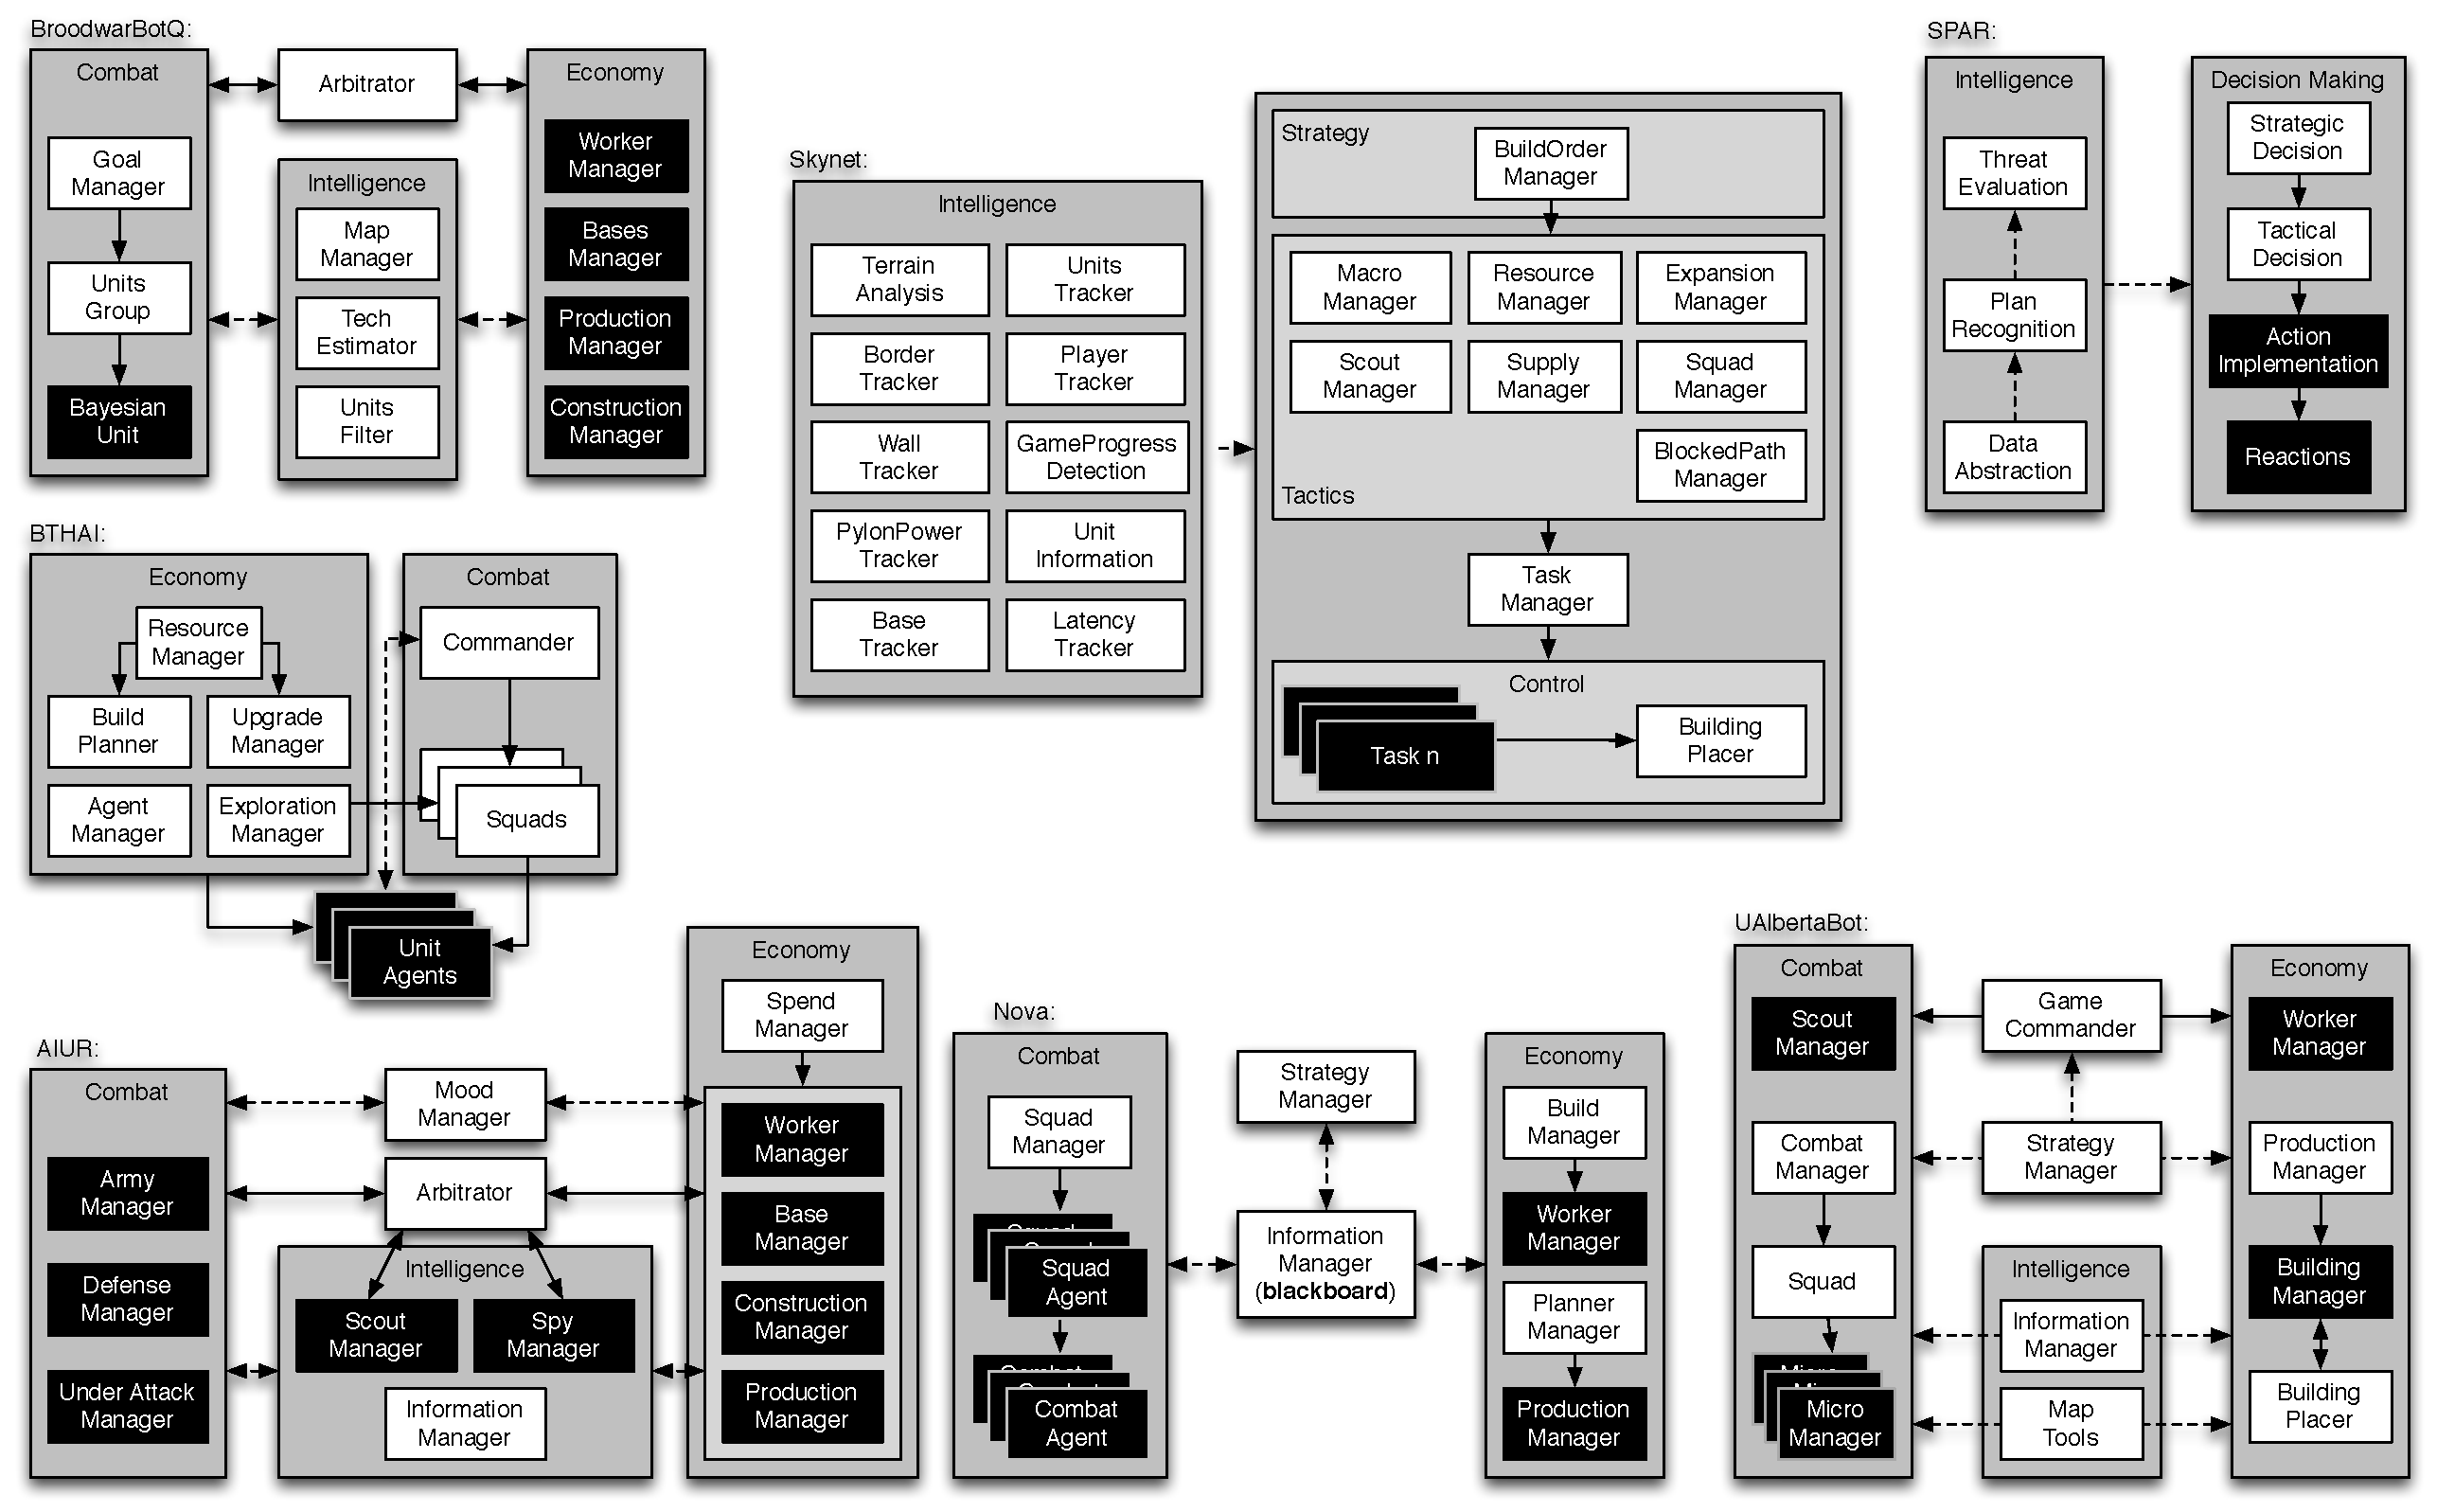
\includegraphics[width=\textwidth]{figures/figure-bot-architectures-wide.pdf}
    \caption{Architecture of 6 Starcraft bots. Modules with black background sent commands directly to Starcraft, dashed arrows represent data flow, and solid arrows represent control.}
    \label{fig:bot-architecture}
\end{figure*}

Figure \ref{fig:bot-architecture} shows some representative examples of the integration architectures used by different bots in the AIIDE and CIG 2011 Starcraft AI competitions \cite{url1,url2}: BroodwarQ \cite{???}, Nova \cite{???}, UAlbertaBot \cite{???}, Skynet \cite{???}, SPAR \cite{???}, and BTHAI \cite{???} (see Section \ref{sec:competition} for a comparison of their performance). Each box represents an individual module with a clearly defined task (only modules with a black background can send actions directly to Starcraft). Dashed arrows represent data flow, and solid arrows represent control (when a module can command another module to perform some task). For example, we can see how SPAR is divided in two sets of modules: {\em situation analysis} and {\em decision making}, the first with three modules dedicated to analyze the current situation of the game, and the later with 4 modules dedicated to exploit that information to decide what to do. We can see how the decision making aspect of SPAR is organized hierarchically, with the higher-level module ({\em strategic decision}) issuing commands to the next module ({\em tactical decision}), which sends commands to the next module ({\em action implementation}), and so on. Only the lower-level modules can send actions directly to Starcraft. 

On the other hand, bots such as NOVA or BroodwarBotQ (BBQ) only use a hierarchical organization for {\em micro-management} (controlling the attack units), but use a decentralized organization for the rest of the bot. In Nova and BBQ, there is a collection of modules that control different aspects of the game (workers, production, construction, etc.). These modules can all send actions directly to Starcraft. In Nova those modules coordinate mostly through writing data in a shared blackboard, and in BBQ they coordinate only when they have to use a shared resource (unit) by means of an arbitrator.

By analyzing the structure of these bots, we can see that there are two main tools that can be used when designing an integration architecture:

\begin{itemize}
\item {\em Abstraction}: complex tasks can be formulated at different levels of abstraction. For example, playing an RTS game can be seen as issuing individual low-level actions to each of the units in the game, or at a higher level, it can be seen as deploying a specific strategy (e.g. a ``BBS strategy'', or a ``Reaver Drop'' strategy). Some bots, reason at multiple levels of abstraction at the same time, making the task of playing Starcraft simpler. Assuming that each module in the architecture of a bot has a goal and determines some actions to achieve that goal, the actions determined by higher-level modules are considered as the goals of the lower level modules. In this way, each module can focus on reasoning at only one level of abstraction, thus, making the problem easier.

\item {\em Divide-and-conquer}: playing a complex RTS, such as Starcraft, requires performing many conceptually different tasks, such as gathering resources, attacking, placing buildings, etc. Assuming each of these tasks can be performed relatively independently and without interference, we can have one module focusing on each of the tasks independently, thus making the problem easier. 
\end{itemize}

If we imagine the different tasks to perform in a complex RTS game in a two-dimensional plane, where the vertical axis represents abstraction, and the horizontal axis represents the different aspects of the game (micro-management, resource gathering, etc.), abstraction can be seen as dividing the space with horizontal lines, whereas divide-and-conquer divides the space using vertical lines.

Different bots, use different combinations of these two tools. Looking back at Figure \ref{fig:bot-architecture}, we can see the following use of abstraction and divide-in-conquer in the bots:

\begin{itemize}
\item BroodwarBotQ: uses abstraction for micro-management, and divide-and-conquer for macro-management and intelligence gathering. To avoid conflicts between modules (since the individual tasks of each of the modules are not completely independent), BBQ uses an arbitrator.
\item Nova: is similar in design as BroodwarBotQ, and uses abstraction for micro-management, and divide-and-conquer for macro-management. The differences are that Nova does not have an arbitrator to resolve conflicts, but has a higher-level module ({\em strategy manager}), which posts information to the blackboard that the rest of modules follow (thus, making use of abstraction).
\item UAlbertaBot: also uses abstraction in micro-management like the previous two bots. But it also uses it in macro-management: as can be seen, the production manager sends commands to the building manager, who is in charge of producing the buildings. This bot also uses divide-and-conquer, and tasks like scouting and resource gathering are managed by separate, independent modules.
\item Skynet: makes extensive use of both abstraction and divide-and-conquer. Considering the decision making component of Skynet, we can see a high level module that issues commands to a series of tactics modules. The collection of tactic modules queue {\em tasks} (that are analogous to the abstract actions used in SPAR). Each different task has a specific low level module that knows how to execute it. Thus, Skynet uses a 3 layered abstraction hierarchy, and uses divide-and-conquer in all levels except the highest.
\item SPAR: only uses abstraction. Its high-level module determines the strategy to use, and the tactical decision module divides it into a collection of {\em abstract actions}, that are executed by the lower-level modules.
\item BTHAI: uses a two-tier abstraction hierarchy, where a collection of high-level modules command a collection of lower-level agents in charge of each of the units. At the high-level, BTHAI uses divide-and-conquer, having multiple high-level modules issuing commands to the lower-level units.
\end{itemize}

Additionally, except for BTHAI, all other agents use divide-and-conquer at a higher-level bot design and divide all the modules into two or three categories: {\em information gathering} and {\em decision}, or {\em information gathering}, {\em micro-management} and {\em macro-management}.

Most bots using divide-and-conquer (except for BBQ and UAlbertaBot), assume that each of the modules can act independently and that their actions can be executed without interference. BBQ and UAlbertaBot use an arbitrator ({\em Game Commander'} in UAlbertaBot) that makes sure that modules do not send contradictory orders to the same unit. However, very little bots handle the problem of how to coordinate resource usage amongst modules, for instance BTHAI uses a first-come-first-serve policy for spending resources, the first module that requests resources is the one that gets them. Nova and Skynet are exceptions, and implement some rudimentary prioritization based on the high level strategy.

One interesting aspect of the five bots described above is that, while all of them are reactive at the lower level (unit control), most if not all of them, are scripted at the highest level of abstraction. BTHAI reads build and squad formations from a predefined script, Nova's {\em Strategy Manager} is a predefined finite-state machine, BBQ's construction manager reads the build order from a predefined script, and Skynet's {\em BuildOrder Manager} is basically a predefined script. Such scripts describe the strategy that the bots will use, however, such strategy is always fixed. One could see this pre-scripting as if each bot defined a ``high-level programming language'' to describe Starcraft strategies, and the bots themselves are just interpreters of such strategy. Compared to current approaches for Chess or Go, this scripting seems a rigid and inflexible, but responds to the much higher complexity of the Starcraft game. An interesting exception to that is UAlbertaBot, which uses a search algorithm in the {\em Production Manager} to find near-optimal build orders. 

In conclusion, we can see that there are two basic tools that can be used in an integration architecture: abstraction and divide-and-conquer, which are widely used by the existing Starcraft bots. 

This section has focused on discussing the architecture of existing Starcraft bots. Let us now focus on what is the state of the art on the techniques used for each of the individual modules used by them.

\subsection{Individual AI Techniques}\label{sec:techniques}

{\color{red} TODO}

\section{Recent Starcraft AI Competitions}\label{sec:competition}

{\color{magenta}

\subsection{CIG 2011}
\label{sec:cig2011}

An initial attempt to run a StarCraft tournament at the Computational
Intelligence in Games conference 2010 suffered from technical problems.
These mainly stemmed from the desire to use evolved, largely untested
maps which proved to look interesting but made the submitted bots crash
so often that it would have been unjustifiable to announce a winner.

At the CIG 2011, the tournament was therefore run with a (secret) selection
of maps used in league play. It was organized by Tobias Mahlmann and Mike
Preuss and attracted 10 bots.

\begin{table*}[htb]
\caption{Bracket A results at CIG 2011, 
qualified for the final round: UAlbertaBot and Skynet.}
\label{tab:correlations}
\begin{small}
\begin{center}
\begin{tabular}{|l|c|c|c|}
\hline
Crashes & games & bot	& wins\\ \hline
0 &	 40 &	 UAlbertaBot &	 33\\
1 &   40 &	 Skynet	  &  31\\
2 &	 40 &	 AIUR	  &  24\\
1 &	 40 &	 Nova	  &  8\\
0 &	 40 &	 LSAI	  &  4\\
\hline
\end{tabular}
\end{center}
\end{small}
\end{table*}




Bracket B

Crashes	 Games	 Bot	 Wins
12	 40	 Xelnaga	 25
3	 40	 BroodwarBotQ	 23
0	 40	 BTHAI	 23
17	 40	 Protoss Beast Jelly	 17
0	 40	 EvoBot	 12
As BroodwarBotQ and BTHAI have the same number of wins, their direct encounter is evaluated which accounted 6 : 4 for the BroodwarBotQ.

Qualified for the final round: Xelnaga and BroodwarBotQ. Note that all qualified bots play Protoss.
Maps used for the first round: (2)MatchPoint 1.3, (4)Fighting Spirit 1.3, iCCupdestination 1.1, iCCup gaia, iCCup great barrier reef

Final Round

The final round was played in a similar mode as each of the first round brackets, using another set of 5 maps (see below), resulting in 30 games for each bot.

Crashes	 Games	 Bot	 Wins
0	 30	 Skynet	 26
0	 30	 UAlbertaBot	 22
3	 30	 Xelnaga	 11
2	 30	 BroodwarBotQ	 1


Here describe the results obtained in the competition comparing the bots.
}



\section{Open Questions in RTS Game AI}\label{sec:questions}

{\color{blue}
Here, describe what is left to be done.
}


\section{Empirical Evidence of What is Missing in Existing Bots}\label{sec:experiments}

{\color{blue}
Here, whatever experiments we want to include to support which aspects of RTS Game AI require more work.
}

\section{Discussion and Conclusions}\label{sec:conclusions}



\section*{Acknowledgments} {\color{blue} This research is partially funded by projects ... and ... }



% Can use something like this to put references on a page
% by themselves when using endfloat and the captionsoff option.
\ifCLASSOPTIONcaptionsoff
  \newpage
\fi

%\begin{thebibliography}{1}
%\end{thebibliography}
\bibliographystyle{IEEEtran}                                                    
\bibliography{survey}

%\begin{IEEEbiographynophoto}{FirstName LastName}
%Biography text here.
%\end{IEEEbiographynophoto}

\begin{IEEEbiography}[{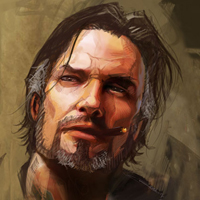
\includegraphics[width=2cm, keepaspectratio]{jim.jpg}}]{Jim Raynor}
Jim Raynor was a Confederate marshal on Mar Sara at the time of the first zerg incursions on that world. He is now with Raynor's Raiders Inc.
\end{IEEEbiography}

\end{document}


In his AIIDE 2010 keynote, Chris Jurnet described the technique XXX, implemented by [COMPANY] in the game YYY \cite{gameurl}
